\section{Results and discussion}

This section presents the results for the proposed Austrian case study for the target year 2050. Four different storylines are investigated covering a wide range of possible future developments of the European and Austrian energy system. Section \ref{res:1} shows the heat generation mix of the low temperature heat supply on the national level. These results are subsequently used for the demonstration of the proposed downscaling methodology. Section \ref{res:2} goes into a higher spatial granularity and shows the heat generation on the sub-region and small-subregion level. Section \ref{res:3} presents the potentials of network-based low temperature heat supply as implication of the four different storylines and European deep decarbonization respectively. Section \ref{res:4} presents the low temperature heat networks on the small sub-region level. Finally, Section \ref{res:5} compares the results of the work with existing low temperature heat networks by using heat density as criteria.

\subsection{Low temperature heat supply in Austria 2050: four different decarbonization scenarios obtained from the H2020 project openENTRANCE}\label{res:1}
This section presents heat generation mix of the low temperature heat supply in Austria for four different storylines which were (\textit{or "are currently"}) developed within the H2020 openENTRANCE project. They are named as follows: \textit{Directed-Transition}, \textit{Societal Commitment}, \textit{Techno-Friendly}, and \textit{Gradual Development}. Whithin each of them, a specific fundamental developement of the energy systems is described while aiming for a sustainable transition of the provision of energy services. Note that the first three storylines consider the achievement of the \SI{1.5}{\degreeCelsius} global warming climate target. The latter storyline (\textit{Gradual Development}) can be interpreted as a more conservative storyline and takes into account the \SI{2.0}{\degreeCelsius} target. In the following, the storylines are briefly described, before the quantitative results of the low temperature heat supply on the national level are presented. For a more detailed description of the storylines, it is referred to \cite{auer2020quantitative} and \cite{auer2020development}. Further informations also are available at the website\footnote{\url{https://openentrance.eu/}} and GitHub.\footnote{\url{https://github.com/openENTRANCE}}.\newline

% Should we add here a table of the storylines with a short description as a quick overview?
% \usepackage{booktabs}
%\begin{table}[H]
%\centering
%\caption{Storylines developed within H2020 openENTRANCE project and their description (further information available on the openENTRANCE website or GITHUB page.).}
%\begin{tabular}{@{}lll@{}}
%\toprule
%Scenario            & Description & Climate target \\ \midrule
%Directed-Transition &             &                \\
%Societal Commitment &             &                \\
%Techno-Friendly     &             &                \\
%Gradual Development &             &                \\ \bottomrule
%\end{tabular}
%\end{table}

The underlying concept of the storylines is a three-dimensional space spanned by the following parameters: technology, policy, and society. Each storyline descibes a specific pathway to reach a decarbonized energy system taking into account a pronounced contribution of two dimensions. Regarding the third dimension, a development is assumed that leads to no significant contribution to the decarbonization of the energy system. The \textit{Directed Transition} storyline looks at a sustainable provision of energy services through strong policy incentives. This becomes necessary because neither the markets nor society adequately push sustainable energy technologies. The \textit{Societal Commitment} storyline achieves a deep decarbonization of the energy system by a strong societal acceptance of the sustainable energy transition. Thereby, decentralized renewable energy technologies together with policy incentives lead to a sustainable supply of energy service needs. Parallel, no fundamental breakthroughs of new clean technologies are within sight. \textit{Techno-Friendly} describes a development of the energy system where a significant market-driven breakthrough of renewable energy technologies give rise to a decarbonization of energy service supply. Alongside, society acceptance supports the penetration of the clean energy technologies and the sustainable transition. \textit{Gradual Development} differs from the other storylines as on the one hand, this storyline only aims for the less ambitios \SI{2.0}{\degreeCelsius} climate target, and on the other hand, a little of each possible sustainable development of the energy system is described here. While all the three dimensions contribute to the decarbonization, they do not push it sufficiently and result in a more conservative storyline than the others.\newline

Table \ref{tab:1} shows the low temperature heat technology generation in Austria for \SI{2050}{} for all four storylines. The values are obtained from the H2020 project openENTRANCE and correspond to modeling results from the open-source model GENeSYS-MODv2.0 \cite{burandt2018genesys}. According to the definition of the storylines, the heat generation by the different technologies vary in some cases significantly (e.g., hydrogen-based low temperature heat generation in \textit{Directed Transition} and \textit{Gradual Development} (\SI{+7.62}{TWh}) or Heat pump (ground) generation in \textit{Techno-Friendly} and \textit{Societal Commitment} (\SI{14.78}{TWh})). Consequently, that share of heat generation which requires heat network infrastructure given the assumptions of this work, also differs (see gray-colored column $\Sigma$).

\newcolumntype{R}[2]{%
	>{\adjustbox{angle=#1,lap=\width-(#2)}\bgroup}%
	l%
	<{\egroup}%
}
\newcommand*\rot{\multicolumn{1}{R{45}{1em}}}
\newcommand*\rots{\multicolumn{1}{R{90}{1em}}}
\definecolor{Gray}{gray}{0.85}

\begin{table} \centering
	\scalebox{0.9}{
	\begin{tabular}{clcccccccc}
		\multicolumn{2}{c}{Heat generation in \SI{}{TWh}} & \rot{Biomass} & \rot{Direct Electric} & \rot{Synthetic gas} & \rot{Heat pump (air)} 
		& \rot{Heat pump (ground)} & \rot{Heat storage} & \rot{Hydrogen} & $\Sigma$\\
		\midrule
		\parbox[t]{2mm}{\multirow{4}{*}{\rotatebox[origin=c]{90}{\small Storyline}}}
		& Directed Transition             & 5.37 & 2.13  & 0.36  & 22.73  & 19.50  & 14.84  & 1.03  & \cellcolor{Gray}25.90\\
		& Societal Commitment               & 5.37 & 1.98 & 1.35 & 15.71 & 21.47 & 10.58 & 2.18 & \cellcolor{Gray}29.02\\
		& Techno-Friendly              & 5.37 & 1.53  & 2.79  & 25.95  & 6.69 & 16.36 & 7.43  & \cellcolor{Gray}19.49\\
		& Gradual Development & 5.37 & 1.81 & 5.35 & 9.68 & 21.21 & 15.57  & 8.65 & \cellcolor{Gray}35.23\\
		\bottomrule
	\end{tabular}}
	\caption{Low temperature heat technology generation in Austria for \SI{2050}{} and the four different storylines. Values obtained from the H2020 project openENTRANCE and GENeSYS-MOD.}
	\label{tab:1}
\end{table}

\subsection{Decarbonized low temperature heat technology generation on different spatial granularity levels}\label{res:2}
In this section, results of the low temperature heat technology generation obtained for the region/country, sub-region, and small sub-region level are presented and discussed. As already mentioned above, the sub-region level corresponds to small political districts and the small sub-region level to (small) municipalities. Note that in Europe, the NUTS classification (Nomenclature of territorial units for statistics) and corresponding regional codes are used within the computations and illustrations of the results. Accordingly, the region/country level is defined within the NUTS classification by the NUTS0 code (e.g., AT for Austria), the sub-region level by the NUTS3 code (e.g., AT127 for South Viennese environs), and the small sub-region level by the local administrative units (LAU) code (e.g., AT127|Laxenburg for the municipality of Laxenburg).\newline

Figure \ref{fig:res1} shows the low temperature heat technology generation on different NUTS levels. Conseptualizing the different subfigures (in Figure \ref{fig:res1}) as 2D-matrix-like structure, each row represents results obtained from data from a different storyline. The horizontal dimension covers the different spatial resolutions, whereby the level of spatial details increases from the left to the right. On the far left, the low temperature heat generation on the country level is presented. In the middle, two different illustrative sub-regions are presented. The rural sub-region (NUTS3 code AT121 (Mostviertel-Eisenwurzen)) shows high shares of heat pumps (air sourced) and small-scale heat storage systems. In addition, synthetic gas and direct electric heating systems supply the low temperature heat demand. In contrast, the urban sub-region (NUTS3 code AT127 (South Viennese environs)) is mainly supplied by ground sourced heat pumps, biomass, and hydrogen. Moreover, air-sourced heat pumps and again heat storage supply the demand. In particular, the shares of heat generation technologies that require network infrastructure are highlighted and marked by the blue-colored edge. On the very right, an example of the resulting low temperature heat network on the small sub-region level for the four different storylines is presented. In the four subfigures presenting centralized heat networks (each for one storyline), the size of the points indicates the amount of centralized low temperature heat supply in a specific small sub-region. The comparably high demand in the \textit{Gradual Development} storyline results in an extensive low temperature heat network infrastructure/topology (see lower right subfigure in Figure \ref{fig:res1}). In contrast, the other three centralized heat networks are characterized by fewer (less supplied small sub-regions) and smaller points (less supplied heat demand by the centralized heat network).

\begin{sidewaysfigure}
	\centering
	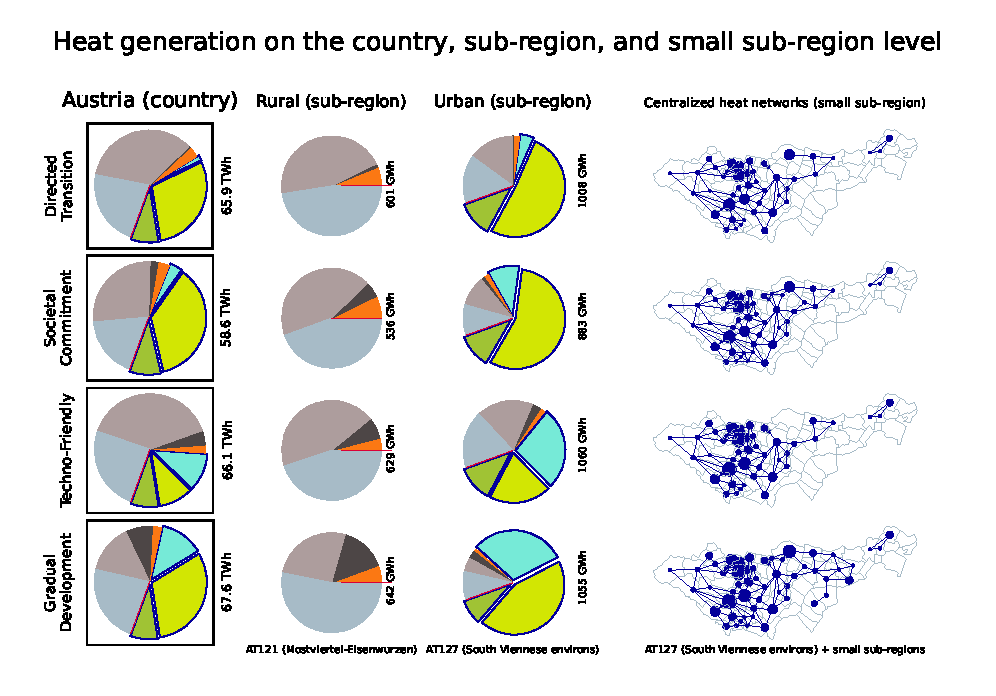
\includegraphics[width=1\linewidth]{figures/4_Results/Spatial_results.eps}
	\caption{Low temperature heat technology generation on different spatial granularity levels for the four different storylines. left: heat technology generation mix on the country level. middle: comparison of technologies supplying the low temperature heat demand in a rural and urban sub-region. right: Centralized heat network topology (size of the points represent the amount of local heat demand supplied by the centralized heat network)}
	\label{fig:res1}
\end{sidewaysfigure}
\newpage
\subsection{Austrian sub-regions with high potentials for centralized low temperature heat supply resulting from aiming the decarbonization}\label{res:3}
As already indicated by Figure \ref{fig:res1}, the results show that there is only a limited number of sub-regions in Austria that have sufficient population and thus heat density to allowing centralized heat supply. Figure \ref{fig:res2} shows a heatmap for centralized heat supply in Austria 2050. Thereby, the spatial granularity corresponds to sub-regions or the NUTS3 level respectively. The corresponding six sub-regions are supplied by the heat networks, independent of the storylines. However, the individual quantities of centralized heat supply per sub-region differ between the storylines (see also the heat technology generation mix of the sub-region AT127 in the center of Figure \ref{fig:res1} as an example for this). In addition, it is important to note here two things: Firstly, Figure \ref{fig:res2} only shows the quantity of centralized heat supply per sub-region. At the same time, heat generation technologies which are not fixed to a central heat distribution network also supply some parts of the heat demand there (see again the heat technology generation mix of the sub-region AT127 in the center of Figure \ref{fig:res1} as an example). Therefore, in those sub-regions in Figure \ref{fig:res2} that are colored completely white which indicated no supply by a centralized heat network, results show that the heat demand in these regions is completely covered by technologies that do not require a heat network infrastructure. And secondly, as expected, the areas seen in Figure \ref{fig:res2} which are projected to have centralized heat supply are those with the highest population density. The range of population density there varies between \SI{229}{persons \per \kilo\metre^2} (AT323 - Salzburg and sourroundings) and \SI{5124}{persons \per \kilo\metre^2} (AT130 - Vienna). As indicated in Figure \ref{fig:res2} (orange box), in the following section, the marked sub-regions are further spatially dissaggregated and, subsequently, their heat network topology is analyzed. 

\begin{sidewaysfigure}
	\centering
	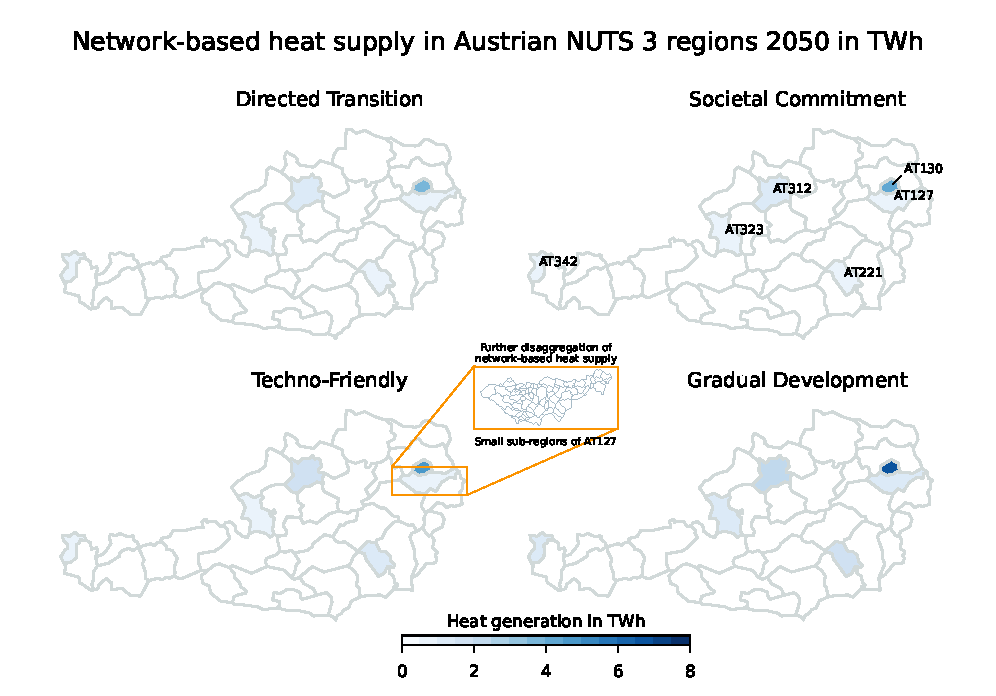
\includegraphics[width=1\linewidth]{figures/4_Results/Heatmap.eps}
	\caption{Centralized low temperature heat supply in Austria 2050. Six sub-regions provide sufficient values of population density to supply parts of the low temperature heat demand by heat networks. The remaining heat demand is supplied by on-site heat technology options. }
	\label{fig:res2}
\end{sidewaysfigure}

\newpage
\subsection{Low temperature heat network topology on the small sub-region level}\label{res:4}
This section analyzes the heat network topology of those regions, that provide sufficient characteristic in terms of population density for centralized heat supply. Figure \ref{fig:res3} shows the boxplot of the distribution of benchmark indicator value for the sub-region AT127 (including all small sub-regions). The number of small sub-regions supplied by the centralized heat network is plotted on the horizontal axis. Note that this number decreases from left to right. It becomes visible that by removing small sub-regions, namely iteratively those with the smallest indicator value, the mean indicator value of the entire remaining heat network increases. In addition, the maximum value of the indicator also increases from under 1.64 to over 7.16. In the present example, the number of small sub-regions supplied by the centralized heat network decreases from \SI{75}{} to \SI{47}{} (\SI{-37.3}{\%}). The iterative reduction of supplied small sub-regions does not necessarily result in a contiguous graph. For example, three small sub-regions form a subgraph that is separate from the other network (see upper right in the green box in Figure \ref{fig:res3}).\newline

The results discussed above suggest that reducing the number of small sub-regions supplied by the centralized heat network increase the indicator value and thus the efficiency of the heat network topology. Simultaneously, this also increases the heat density of the supply area. In the following subsection, the obtained heat density values of the heat networks are compared with existing values and today's minimum required values for centralized heat networks.

% Is this figure intuitive? in particular the x-axis ==> do we need here a second axis that indicates the iterative steps of the algorithm?
\begin{sidewaysfigure}
	\centering
	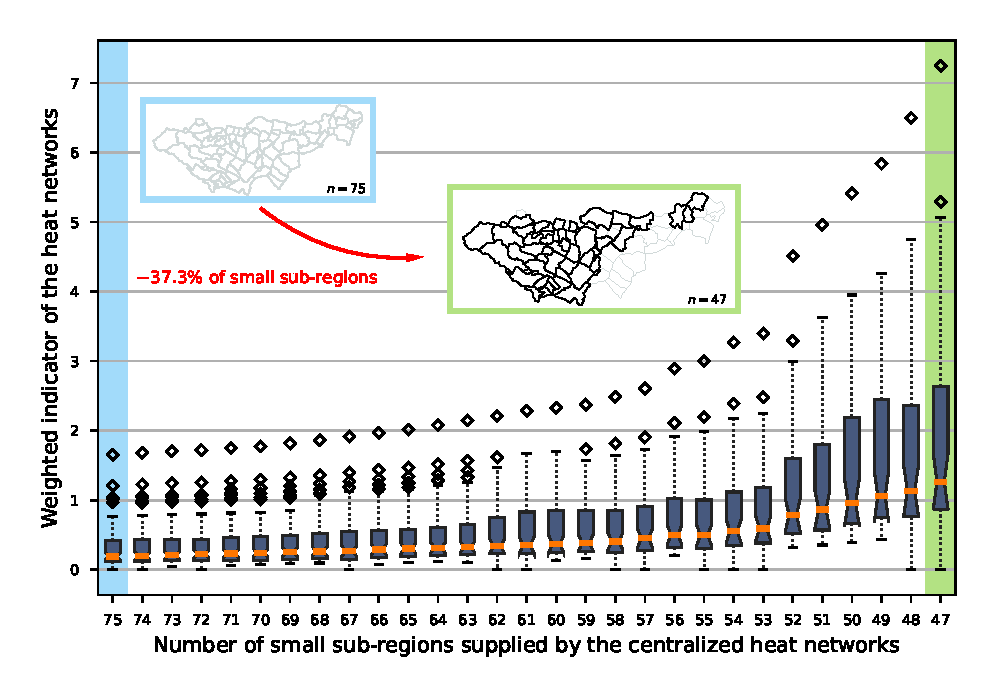
\includegraphics[width=1\linewidth]{figures/4_Results/boxplot.eps}
	\caption{Weighted indicator value of the low temperature heat network at the sub-region AT127 (South Viennese environs) for different numbers of areas supplied by the centralized heat networks.}
	\label{fig:res3}
\end{sidewaysfigure}
\newpage
\subsection{Comparison of existing and future projections of low temperature heat networks using heat and population density}\label{res:5}
This section synthesizes the results in the context of heat density values of centralized heat networks and compares the obtained future projections of sustainable centralized heat supply with current minimum required heat density standards of heat networks. Figure \ref{fig:res4} shows the heat density of low temperature heat networks for different the different proposed downscaling techniques and the four different storylines. The population density is shown on the horizontal axis. The black triangles mark the minimum required heat density for today's centralized heating networks at a connection rate of \SI{90}{\%} in Austria.\footnote{See in this context for example \url{http://www.austrian-heatmap.gv.at/karte/}.} The circles ($\bullet$) mark the default downscaling with only population as criterion. Therefore, the heat density of the sub-regions increases linearly with the population density (see also the zoomed out area in the left subfigure with population density $\leq 150 \frac{persons}{km^2}$). The diamonds ($\blacklozenge$) mark the heat density values obtained by Algorithm 1 (and thus without supply area reduction). As a result, the heat density per sub-region increases (see the zoomed out area in the middle subfigure with population density $\leq 500 \frac{persons}{km^2}$). The stars ($\bigstar$) mark the heat density resulting by Algorithm 2. In order to highlight the effects of the different downscaling techniques, the differences of the resulting heat densities to today's minimum required values is shown for a sub-region by the three green bars for the \textit{Techno-Friendly} storyline. As the comparison of the green bars shows, the difference is again significantly reduced by applying Algorithm 2.

\begin{sidewaysfigure}
	\centering
	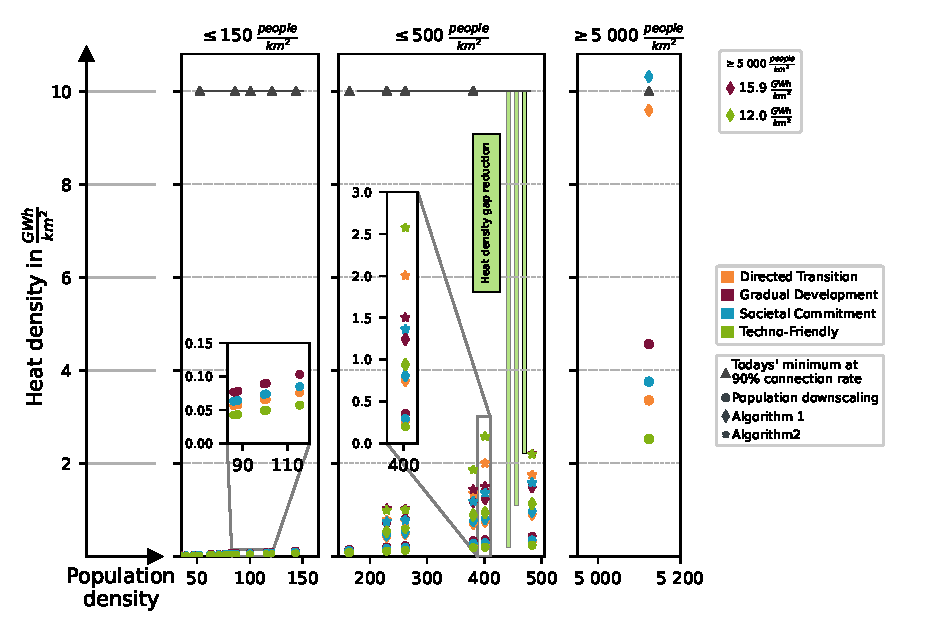
\includegraphics[width=1\linewidth]{figures/4_Results/Heat_density_gap.eps}
	\caption{Heat densities for different population densities, decarbonization storylines, and downscaling techniques. Reducing significantly the gap between today's minimum required heat density (\SI{10}{\frac{GWh}{km^2}} at a connection rate of \SI{90}{\%}) by Algorithm 2 in comparison with default population-based downscaling.}
	\label{fig:res4}
\end{sidewaysfigure}
